\documentclass[12pt]{article}
\usepackage[english]{babel}
\usepackage{natbib}
\usepackage{url}
\usepackage[utf8x]{inputenc}
\usepackage{amsmath}
\usepackage{graphicx}
\graphicspath{{img/}}
\usepackage{parskip}
\usepackage{fancyhdr}
\usepackage{listings}
\usepackage{vmargin}
\setmarginsrb{3 cm}{2.5 cm}{3 cm}{2.5 cm}{1 cm}{1 cm}{1 cm}{1 cm}

\title{Lab Report on\\ Basic Point Operation on Image }								% Title
\author{Rabi Raj Khadka }								% Author
\date{\today}											% Date


\makeatletter
\let\thetitle\@title
\let\theauthor\@author
\let\thedate\@date
\makeatother

\pagestyle{fancy}
\fancyhf{}
\rhead{\theauthor}
\lhead{\thetitle}
\cfoot{\thepage}

\begin{document}

%%%%%%%%%%%%%%%%%%%%%%%%%%%%%%%%%%%%%%%%%%%%%%%%%%%%%%%%%%%%%%%%%%%%%%%%%%%%%%%%%%%%%%%%%

\begin{titlepage}
	\centering
    \vspace*{0.2 cm}
    
\includegraphics[scale = 0.3]{kheclogo.jpg}\\[1.0 cm]	% University Logo
    \textsc{\LARGE Khwopa Engineering College}\\[2.0 cm]	% University Name
	\textsc{\Large Course Code :BEG 475 IP}\\[0.5 cm]				% Course Code
	\textsc{\large Image Processing and Pattern Recogntiion}\\[0.5 cm]				% Course Name
	\rule{\linewidth}{0.2 mm} \\[0.4 cm]
	{ \huge \bfseries \thetitle}\\
	\rule{\linewidth}{0.2 mm} \\[1.0 cm]
	% \texttt{Lab Report \#1}
	
	\rule{\linewidth}{0 mm} \\[1.0 cm]

	\begin{minipage}{0.4\textwidth}
		\begin{flushleft} \large
			\emph{Author:}\\
			\theauthor
			\end{flushleft}
			\end{minipage}~
			\begin{minipage}{0.4\textwidth}
			\begin{flushright} \large
			\emph{Roll  Number:} \\
			700324									% Your Student Number
		\end{flushright}
	\end{minipage}\\[2 cm]
	
	{\large \thedate}\\[2 cm]
 
	\vfill
	
\end{titlepage}

%%%%%%%%%%%%%%%%%%%%%%%%%%%%%%%%%%%%%%%%%%%%%%%%%%%%%%%%%%%%%%%%%%%%%%%%%%%%%%%%%%%%%%%%%

\tableofcontents
\pagebreak

%%%%%%%%%%%%%%%%%%%%%%%%%%%%%%%%%%%%%%%%%%%%%%%%%%%%%%%%%%%%%%%%%%%%%%%%%%%%%%%%%%%%%%%%%

\section{Theory:}
\subsection{Image and Its Type}
An image is defined as a 2D function f(x,y) where (x,y) is that spatial co-ordinate. An image consists of 3 elements\\
1. picture elements like luminance and chrominance\\
2. image elements like lines and segments\\
3. pels of pixel composed of RGB or B/W\\

There are different types of images\\
1. Binary image\\
It contains only 1 bit color information intensity value either0 or 1. These are helpful in various scientific areas like medical X-ray, B/W images etc\\

2. Gray-Scale image\\
It have 8-bit quantized intensity levels between 0 and 1. It have 0-255 different intensity to represent an image.\\

3. Color image\\
It contains 3 picture elements R,G,B each having 8-bit quantized intensity levels for each pixel values to form a color image. Each pixel contains $2^{24}$ bit image information.\\

4. Indexed image\\
It contains only index of the pixel that should be mapped on color pallete of an imaging devices rather than intensity info. It is device independent. For example a TIFF image


\subsection{Point Operations on Image}

1. Negative\\
2. Log Transformation\\
3. Power Transformation\\
4. Intensity Level Slicing\\
5. Bit Plane SLicing\\

\subsection{Functions for Image Operation on Matlab}
1. imread()\\
A = imread(filename) reads the image from the file specified by filename, inferring the format of the file from its contents. If filename is a multi-image file, then imread reads the first image in the file.\\\\
2. imwrite()\\
imwrite(A,filename) writes image data A to the file specified by filename, inferring the file format from the extension. imwrite creates the new file in your current folder. The bit depth of the output image depends on the data type of A and the file format.\\\\
3. imshow()\\
imshow(I) displays image I in a Handle Graphics® figure, where I is a grayscale, RGB (truecolor), or binary image. For binary images, imshow displays pixels with the value 0 (zero) as black and 1 as white. imshow optimizes figure, axes, and image object properties for image display.\\\\
4. rgb2gray()\\
I = rgb2gray(RGB) converts the truecolor image RGB to the grayscale intensity image I. The rgb2gray function converts RGB images to grayscale by eliminating the hue and saturation information while retaining the luminance.\\\\
5. im2bw()\\
BW = im2bw(I, level) converts the grayscale image I to a binary image. The output image BW replaces all pixels in the input image with luminance greater than level with the value 1 (white) and replaces all other pixels with the value 0 (black). Specify level in the range [0,1]. \\\\

\pagebreak

\section{Code Description}
Point Operations on Image \\
\lstinputlisting[language=Matlab]{labtwo.m}





\pagebreak

\section{Result and Discussion}
The original image is converted into different forms like GrayScale image, B/W image and Negative image using the basic MATLAB functions like$$  rgb2gray(image); , im2bw(image); and (255 - image) $$
Final output is generated in the single figure with 6 diferent images as below:\\

\emph{Output:}\\

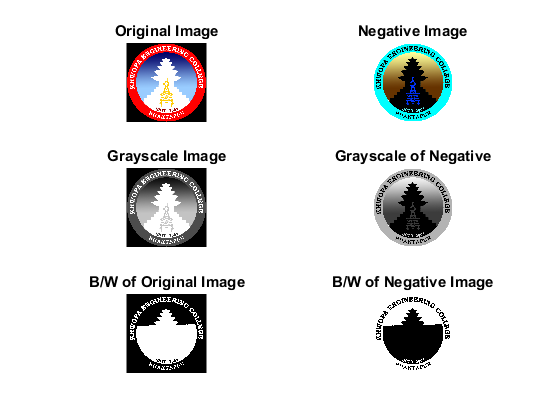
\includegraphics[scale =1.0]{output_labtwo_1.png}







\pagebreak

\section{Conclusion}
Hence, \\
We are familiarized with the  basic image operations using the MATLAB.
\newpage
%\bibliographystyle{plain}
%\bibliography{biblist}

\end{document}